\documentclass{article}

\usepackage{color,amsmath,amssymb,graphicx,fancyhdr,amsfonts,amsthm,verbatim,bbold,environ}
\usepackage{hyperref}
\usepackage{mkolar_definitions}
\usepackage{multirow}
\usepackage{diagbox}
\usepackage{longtable,booktabs}
\usepackage[left=2cm,top=2cm,right=2cm]{geometry}
\usepackage{listings}
% \numberwithin{algorithm}{section}


\newcommand{\tightlist}{%
  \setlength{\itemsep}{0pt}\setlength{\parskip}{0pt}}


%%%%%%%%%%%%%%%%%%%%%%%%%%%%%
\newcommand{\tta}{\theta}
\newcommand{\lag}{\left\langle}
\newcommand{\rag}{\right\rangle}
\newcommand{\lnorm}{\left\|}
\newcommand{\rnorm}{\right\|}
%%%%%%%%%%%%%%%%%%%%%%%%%%%%%
\usepackage[no-math]{fontspec}

\newfontfamily\monaco{Menlo}
\lstset{basicstyle=\footnotesize\monaco,breaklines=true}


\usepackage[ruled,lined,boxed,linesnumbered]{algorithm2e}


\title{EE357 Computer Networks Assignment 3}
\author{Zhou Litao 518030910407 F1803016}
\date{\today , Spring Semester}
\begin{document}
\maketitle

%%%%%%%%%%%%%%%%%%%%%%%%%%%%%%%%%%%%%%%%%%
%%%%%%%%%%%%%                 %%%%%%%%%%%%
%%%%%%%%%%%%%    EXERCISE 1   %%%%%%%%%%%%
%%%%%%%%%%%%%                 %%%%%%%%%%%%
%%%%%%%%%%%%%%%%%%%%%%%%%%%%%%%%%%%%%%%%%%
\begin{exercise}[]{Suppose a process in Host C has a UDP socket with port number 6789. Suppose both Host A and Host B each send a UDP segment to Host C with destination port number 6789. Will both of these segments be directed to the same socket at Host C? If so, how will the process at Host C know that these two segments originated from two different hosts?}
  \begin{solution}
  \par{~}
  Yes, both segments will be directed to the same socket. To discriminate between the two received segments, the operating system will provide the process with the IP addresses of the source of segment so that application process can know the origins of the two segments.
  \end{solution}
  \label{ex1}
\end{exercise}


%%%%%%%%%%%%%%%%%%%%%%%%%%%%%%%%%%%%%%%%%%
%%%%%%%%%%%%%                 %%%%%%%%%%%%
%%%%%%%%%%%%%    EXERCISE 2   %%%%%%%%%%%%
%%%%%%%%%%%%%                 %%%%%%%%%%%%
%%%%%%%%%%%%%%%%%%%%%%%%%%%%%%%%%%%%%%%%%%
\begin{exercise}[]{(15 points) Suppose Client A initiates a Telnet session with Server S. At about the same time, Client B also initiates a Telnet session with Server S. Provide possible source and destination port numbers for

    1. The segments sent from A to S.

    2. The segments sent from B to S.
    
    3. The segments sent from S to A.
    
    4. The segments sent from S to B.
    
    5. If A and B are different hosts, is it possible that the source port number in the segments from A to S is the same as that from B to S?
    
    6. How about if they are the same host?}
  \begin{solution}
  \par{~}
  \begin{enumerate}
      \item Source can be arbitrary for A and the destination port of S is usually 23 (well-known port for Telnet).
      \item Source can be arbitrary for B and the destination port of S is usually 23 (well-known port for Telnet).
      \item Source of S should be 23 and destination can be arbitrary for A (the same with the port number in 1).
      \item Source of S should be 23 and destination can be arbitrary for B (the same with the port number in 2).
      \item Yes. It can be possible.
      \item No. OS will ensure that no ports are simultaneously taken by two clients.
  \end{enumerate}
  \end{solution}
  \label{ex2}
\end{exercise}


%%%%%%%%%%%%%%%%%%%%%%%%%%%%%%%%%%%%%%%%%%
%%%%%%%%%%%%%                 %%%%%%%%%%%%
%%%%%%%%%%%%%    EXERCISE 3   %%%%%%%%%%%%
%%%%%%%%%%%%%                 %%%%%%%%%%%%
%%%%%%%%%%%%%%%%%%%%%%%%%%%%%%%%%%%%%%%%%%
\begin{exercise}[]{(5 points) Describe why an application developer might choose to run an application over UDP rather than TCP.}
  \begin{solution}
  \par{~}
  If the application does not pose demands on reliable data transfer, but cares more about efficiency in transmission (such as streaming media, teleconferencing, DNS, Internet telephony), then UDP might be preferred.  
  \end{solution}
  \label{ex3}
\end{exercise}


%%%%%%%%%%%%%%%%%%%%%%%%%%%%%%%%%%%%%%%%%%
%%%%%%%%%%%%%                 %%%%%%%%%%%%
%%%%%%%%%%%%%    EXERCISE 4   %%%%%%%%%%%%
%%%%%%%%%%%%%                 %%%%%%%%%%%%
%%%%%%%%%%%%%%%%%%%%%%%%%%%%%%%%%%%%%%%%%%
\begin{exercise}[]{(10 points) Considering the TCP 32-bit sequence number. How long will the sequence number will be used up when (Note: For TCP, each byte has a unique sequence number.)

    1. The line is 56-kbps.

    2. The line is 10-Mbps.

    3. The line is 1 Gbps.

    4. Suppose a packet can stay in Internet for 1 minute at most. Do you think 32-bit sequence number is enough for 1Gbps network? If not enough, how TCP deal with this problem?
    }
  \begin{solution}
  \par{~}
  There are $2^32$ sequence numbers available
  \begin{enumerate}
      \item After $\frac{2^32}{56\times 2^10 / 8} = 585.14$s, the sequence number will be used up.
      \item After $\frac{2^32}{10\times 2^10 \times 2^10 / 8} = 3276.8$s, the sequence number will be used up.
      \item After $\frac{2^32}{1\times 2^10\times 2^10 \times 2^10 / 8} = 32$s, the sequence number will be used up.
      \item Not enough. TCP deals with this problem by using sequence numbers again and again. Since TCP sequence number value may wrap around the 32-bit boundary, so all sequencing is done modulo $2^{32}$. In this case, new packets can be resent using old sequence numbers starting from zero. 
  \end{enumerate}
  \end{solution}
  \label{ex4}
\end{exercise}


%%%%%%%%%%%%%%%%%%%%%%%%%%%%%%%%%%%%%%%%%%
%%%%%%%%%%%%%                 %%%%%%%%%%%%
%%%%%%%%%%%%%    EXERCISE 5   %%%%%%%%%%%%
%%%%%%%%%%%%%                 %%%%%%%%%%%%
%%%%%%%%%%%%%%%%%%%%%%%%%%%%%%%%%%%%%%%%%%
\begin{exercise}[]{Problem 5 (10 points) We have said that an application may choose UDP for a transport protocol because UDP offers finer application control (than TCP) of what data is sent in a segment and when.
    
    1. Why does an application have more control of what data is sent in a segment? 
    
    2. Why does an application have more control on when the segment is sent?}
  \begin{solution}
  \par{~}
  \begin{enumerate}
      \item Because UDP is simply a no-frills extension of “best-effort” IP, and the simplicity in UDP implementation makes it transmit whatever message the application layer gives. TCP, on the other hand, may not necessarily put a single message from application layer into one TCP segment. Therefore, an application has more control of what data is sent in a segment with UDP.
      \item In TCP, it ensures flow control and congestion control. Therefore, when the network layer is in traffic, the message may be delayed by TCP. By contrast, UDP does not have such controls and will try it best to send messages from the application layer. Therefore, UDP has more control on when the segment is sent.
  \end{enumerate}
  \end{solution}
  \label{ex5}
\end{exercise}


%%%%%%%%%%%%%%%%%%%%%%%%%%%%%%%%%%%%%%%%%%
%%%%%%%%%%%%%                 %%%%%%%%%%%%
%%%%%%%%%%%%%    EXERCISE 6   %%%%%%%%%%%%
%%%%%%%%%%%%%                 %%%%%%%%%%%%
%%%%%%%%%%%%%%%%%%%%%%%%%%%%%%%%%%%%%%%%%%
\begin{exercise}[]{(20 points) Compare GBN, SR, and TCP (no delayed ACK). Assume that the timeout values for all three protocols are sufficiently long such that 5 consecutive data segments and their corresponding ACKs can be received (if not lost in the channel) by the receiving host (Host B) and the sending host (Host A) respectively. Suppose Host A sends 5 data segments to Host B, and the 2nd segment (sent from A) is lost. In the end, all 5 data segments have been correctly received by Host B.

    1. How many segments has Host A sent in total and how many ACKs has Host B sent in total? What are their sequence numbers? Answer this question for all three protocols.

    2. If the timeout values for all three protocol are much longer than 5 RTT, then which protocol success fully delivers all five data segments in shortest time interval?}
  \begin{solution}
  \par{~}
  \begin{enumerate}
      \item For GBN, A sent 9 segments and B sent 8 ACKs. For SR, A sent 6 segments abd B sent 5 ACKs. For TCP, A sent 6 segments abd B sent 5 ACKs. The details of the numbers can be found in Figure \ref{fig:ex6}.
      \begin{figure}[hb]
        \begin{center}
        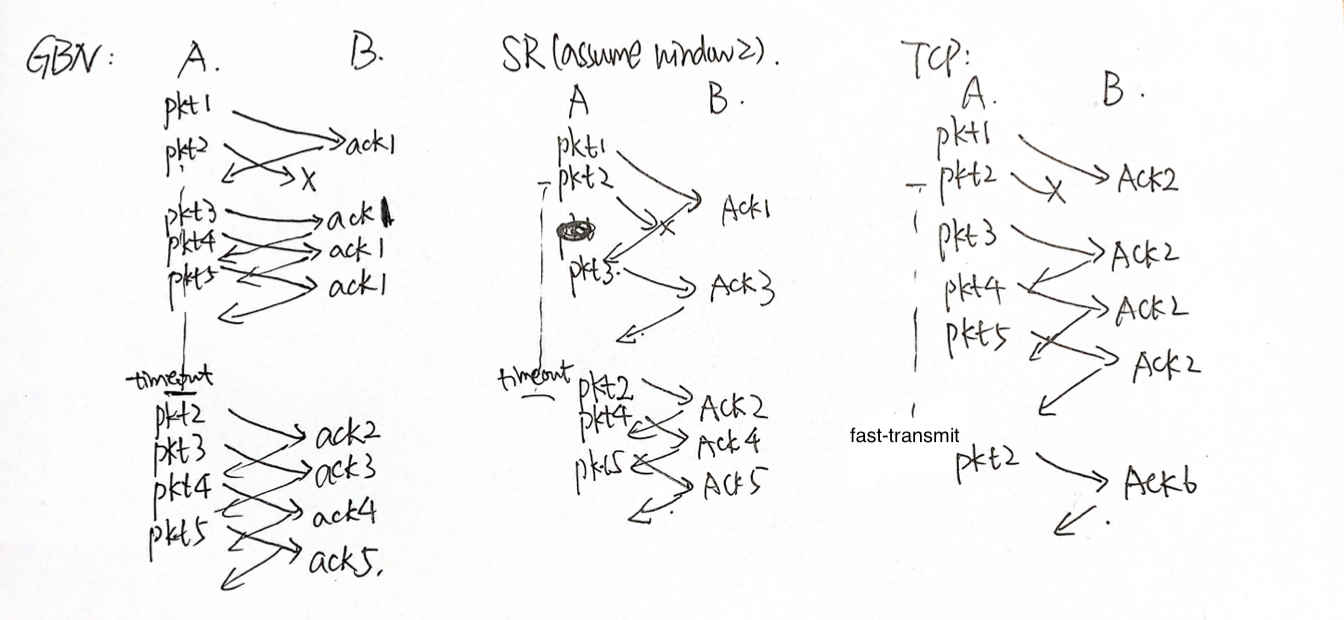
\includegraphics[width=12cm]{img/ass3/ex6}
        \caption{Solution for Exercise \ref{ex6}}
        \label{fig:ex6}
        \end{center}
      \end{figure}
      \item TCP. GBN transfer more packets than TCP. SR has to wait until pkt2 is timeout so that it could continue sending packets next to the current window. But TCP uses fast-retransmit so that it does not have to wait for timeout.
  \end{enumerate}
  \end{solution}
  \label{ex6}
\end{exercise}




%%%%%%%%%%%%%%%%%%%%%%%%%%%%%%%%%%%%%%%%%%
%%%%%%%%%%%%%                 %%%%%%%%%%%%
%%%%%%%%%%%%%    EXERCISE 7   %%%%%%%%%%%%
%%%%%%%%%%%%%                 %%%%%%%%%%%%
%%%%%%%%%%%%%%%%%%%%%%%%%%%%%%%%%%%%%%%%%%
\begin{exercise}[]{ (20 points) Consider Figure \ref{fig:ex7}. Assuming TCP Reno is the protocol experiencing the behavior shown above, answer the following questions. In all cases, you should provide a short discussion justifying your answer.

    1. Identify the intervals of time when TCP slow start is operating.


    2. After the 16th transmission round, is segment loss detected by a triple duplicate ACK or by a timeout?

    3. After the 22nd transmission round, is segment loss detected by a triple duplicate ACK or by a timeout?

    4. What is the initial value of ssthresh at the first transmission round?

    5. What is the value of ssthresh at the 18th transmission round?

    6. What is the value of ssthresh at the 24th transmission round?

    7. During what transmission round is the 70th segment sent?

    8. Assuming a packet loss is detected after the 26th round by the receipt of a triple duplicate ACK, what will be the values of the congestion window size and of ssthresh?

    9. Suppose TCP Tahoe is used (instead of TCP Reno), and assume that triple duplicate ACKs are received at the 16th round. What are the ssthresh and the congestion window size at the 19th round?

    \begin{figure}[hb]
      \begin{center}
      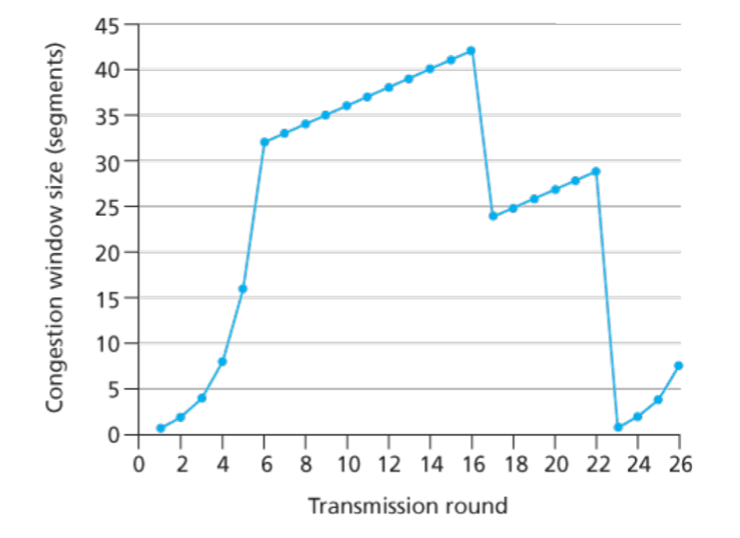
\includegraphics[width=12cm]{img/ass3/ex7}
      \caption{TCP window size as a function of time}
      \label{fig:ex7}
      \end{center}
    \end{figure}
    }
  \begin{solution}
  \par{~}

  \begin{enumerate}
      \item 0 - 4 and 23 - 26 are slow start intervals.
      \item Duplicate ACK, because cwnd is cut in half window and added in 3 MSS.
      \item Timeout, because slow start begins again.
      \item 32. The value should be the time where cwnd begins grow linearly. The cwnd at interval 6 is the ssthresh 32.
      \item 21, because at 17th round, the cwnd is 24 = ssthresh + 3.
      \item 14, should be half of the cwnd at 23th round.
      \item The seventh interval, because the number of previous sent packets is 1 + 2 + 4 + 8 + 16 + 32 = 63.
      \item The cwnd should be 7 and ssthresh should be 4. At this inverval the cwnd should originally be 16, which is larger than the original ssthresh, so it will respond to the triple ACK and transforms into fast recovery state.
      \item 4. Because TCP Tahoe will reduce the cwnd to 1 at the 17th round and begin cold starting.
  \end{enumerate}
  \end{solution}
  \label{ex7}
\end{exercise}


%%%%%%%%%%%%%%%%%%%%%%%%%%%%%%%%%%%%%%%%%%
%%%%%%%%%%%%%                 %%%%%%%%%%%%
%%%%%%%%%%%%%    EXERCISE 8   %%%%%%%%%%%%
%%%%%%%%%%%%%                 %%%%%%%%%%%%
%%%%%%%%%%%%%%%%%%%%%%%%%%%%%%%%%%%%%%%%%%
\begin{exercise}[]{Host A is sending an enormous file to Host B over a TCP connection. Over this connection there is never any packet loss and the timers never expire. Denote the transmission rate of the link connecting Host A to the Internet by R bps. Suppose that the process in Host A is capable of sending data into its TCP socket at a rate S bps, where S = 10 R. Further suppose that the TCP receive buffer is large enough to hold the entire file, and the send buffer can hold only one percent of the file. What would prevent the process in Host A from continuously passing data to its TCP socket at rate S bps? TCP flow control? TCP congestion control? Or something else? Elaborate.}
  \begin{solution}
  \par{~} Neither. Since TCP receiver buffer can always hold the data, the receiver's buffer will never be full. Thus TCP flow control will not affect the transmission rate. Furthermore, since the link has larger transmission rate and no packets will be lost, TCP congestion control will not be triggered at a transmission rate smaller than R bps. It is the limited size of Host A's buffer that prevents the transmission rate reaching S bps, because once the buffer is full, the transmission has to be blocked by the Internet transmission rate R which is smaller than S.
  \end{solution}
  \label{ex8}
\end{exercise}


\end{document}